\documentclass{report}
\usepackage[margin=1in, paperwidth=8.5in, paperheight=11in]{geometry}
%Math packages%
\usepackage{amsmath}
\usepackage{amssymb}
\usepackage{amsthm}
%Spacing%
\usepackage{setspace}
\onehalfspacing
%Lecture number%
\newcommand{\lectureNum}{16}
%Variables - Date and Course%
\newcommand{\curDate}{February 8, 2017}
\newcommand{\course}{MATH 239}
\newcommand{\instructor}{Luke Postle}
%Defining the example tag%
%\theoremstyle{definition}%
\newtheorem{ex}{Example}[section]
%Setting counter given the lecture number%
\setcounter{chapter}{\lectureNum{}}
%Package for drawing graphs%
\usepackage{tikz}
\usepackage{verbatim}
\usetikzlibrary{arrows}

\begin{document}
%Note title%
\begin{center}
\begin{Large}
\textsc{\course{} | Lecture \lectureNum{}}
\end{Large}
\end{center} 
\noindent \textit{Bartosz Antczak} \hfill
\textit{Instructor: \instructor{}} \hfill
\textit{\curDate{}}
\rule{\textwidth}{0.4pt}

% Actual Notes%
\subsubsection{Review of Last Lecture}
When we \textbf{subdivide} an edge $e=uv$, we delete $e$ and add a new vertex $w$ adjacent to only $u$ and $v$.\\An $H-$subdivision is a graph obtained from $H$ by subdividing edges.\\We also covered an if-and-only-if theorem about planar graphs:
\begin{center}
\textit{G is planar $\iff$ G has no $K_5-$substitution and $K_{3,3}-$substitution}
\end{center}
To decide if $G$ is planar, either give an embedding or give a $K_5-$subdivision or $K_{3,3}-$subdivision. So deciding planarity is in $NP$ and co$-NP$, and actually it's in $P$. There is a linear-time algorithm (but it's complicated so we won't cover it).
\section{Colouring}
Prof. Postle wrote it as ``coloring" because he's American, and he refuses to include a `u' because ``screw you".\\
Let's begin with a question:
\begin{center}
Is there a natural generalization of a bipartite graph? (e.g., a tripartite  graph?)
\end{center}
Recall that if $G$ is bipartite if there exists a bipartition of $V(G)$ into two parts $A$ and $B$ such that no edge has both ends in the same partition.
\subsubsection{Definition | Independent Set}
An \textbf{independent set} $I$ of $G$ is a set of vertices with no edge with both ends in $I$. From this, we can construct another (but equivalent) definition of a bipartition:
\begin{center}
$G$ is bipartite if there exists a partition of $G$ into two parts, each of which is an independent set.
\end{center}
From this, we can define a \textit{tripartite} using the previous definition, except we swap the word ``two" with ``three". However, instead of this definition, we'll use different terminology:
\subsubsection{Definition | K-colouring}
A \textbf{k-colouring} of a graph $G$ is a partition of $V(G)$ into $k$ independent sets.\\
Why do we use this terminology? We can attribute each independent set with a unique colour. This results in no edge having two ends of the same colour.
\subsubsection{Definition | K-colourable}
A graph $G$ is $k-$colourable if there is a $k-$colouring of $G$.\\
From this, we create another theorem:
\begin{center}
\textit{G is bipartite $\iff$ G is 2-colourable}
\end{center}
%TODO include graphs (not difficult)%
\begin{ex}
A 3-colourable graph, with partitions 1, 2, and 3
\end{ex}
\begin{center}
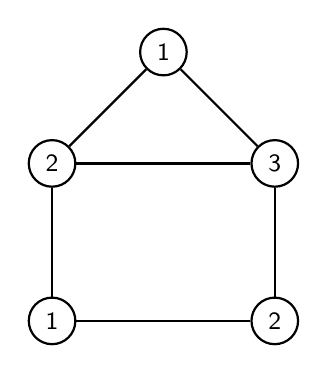
\begin{tikzpicture}[-,auto,node distance=2cm,
                    thick,main node/.style={circle,draw,font=\sffamily\small}]

  \node[main node] (1) {1};
  \node[main node] (2) [below right of=1] {3};
  \node[main node] (3) [below left of=1] {2};
  \node[main node] (4) [below of=3] {1};
  \node[main node] (5) [below of=2] {2};  
  \path[every node/.style={font=\sffamily\large}]
    (1) edge (2)
    	edge (3)
    (2) edge (3)
    	edge (5)
    (4) edge (3)
    	edge (5);
\end{tikzpicture}
\end{center}
\subsubsection{Remark}
If $G$ is $k-$colourable, then $G$ is $m-$colourable for all $m \geq k$ (because the independent sets may be empty).
\subsubsection{Definition | Chromatic number}
The \textbf{chromatic number} of a graph $G$ denoted, $\chi(G)$, is the minimum $k$ such that $G$ is $k-$colourable.
\subsection{Proposition 1}
\begin{center}
\textit{If H is a subgraph of G, then $\chi(H)\leq \chi(G)$}
\end{center}
\subsubsection{Proof of Proposition 1}
Let $k=\chi(G)$ and consider a $k-$colouring of $G$, then that induces a $k-$colouring of $H$, so $\chi(H) \leq k$.
\subsection{Proposition 2}
\begin{center}
\textit{If G contains $k_n$ as a subgraph, then $\chi(G) \geq n$}
\end{center}
\subsubsection{Definition | Clique Number}
Denoted $w(G)$, is the size of a largest complete subgraph of $G$. $\chi(G) \geq w(G)$. This is the \textit{lower bound} on determining the chromatic number of a graph $G$ (recall that this is a greater-than-or-equal-to sign, so the clique number isn't always the chromatic number of a graph $G$).
\begin{ex}
For this graph, $\chi(G) = 4$. Can you match each vertex into their respective partition?
\end{ex}
%TODO draw the graph from EX2%
\begin{center}
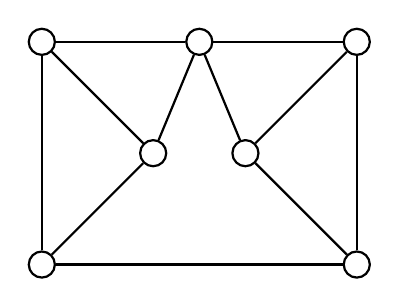
\begin{tikzpicture}[-,auto,node distance=2cm,
                    thick,main node/.style={circle,draw,font=\sffamily\small}]

  \node[main node] (1) {};
  \node[main node] (3) [right of=1] {};
  \node[main node] (2) [left of=1] {};
  \node[main node] (4) [below left of=3] {};
  \node[main node] (5) [below right of=2] {};  
  \node[main node] (6) [below left of=5] {};
  \node[main node] (7) [below right of=4] {};  
  
  \path[every node/.style={font=\sffamily\large}]
    (1) edge (2)
    	edge (3)
    	edge (4)
    	edge (5)
    (5) edge (2)
    	edge (6)
    (4) edge (3)
    	edge (7)
    (7) edge (3)
    (6) edge (7)
    	edge (2);
\end{tikzpicture}
\end{center}
Is deciding if $G$ is $k-$colourable in $NP$? $P$? co$-NP$? It's actually in all three!
\subsubsection{Definition | Maximum Degree}
The \textbf{maximum degree} of a graph $G$, denoted $\Delta(G)$, equals $\mathrm{max}_{v\in V(G)}\, \mathrm{deg}(v)$
\subsection{Theorem 1}
\begin{center}
\textit{$\chi(G) \leq \Delta(G) + 1$ for all graphs G}
\end{center}
\subsubsection{Proof of Theorem 1}
Let $v_1, v_2, \cdots, v_n$ be an arbitrary ordering of $V(G)$. Now colour the vertices in order, where we colour $v_i$ with the lowest colour in $\{1, \cdots, \Delta(G) + 1\}$ that's not used by any neighbours. Such a colour exists because $\mathrm{deg}(G) \leq \Delta(G)$ but there are $\Delta(G) + 1$ colours.
%END%
\end{document}